\section{High Dimensional Bayesian Optimization}
\begin{frame}[c]{High Dimensional Bayesian Optimization}
\begin{itemize}
%    \item Bayesian Optimization success stories:
%    \begin{itemize}
%        \item robotics, planning, recommendation, automatic algorithm configuration etc.
%    \end{itemize}
%    \pause
    \item Issue: BO works best on problems of moderate dimensions $d\leq20$
%    \pause
    \begin{itemize}
        \item Standard GPs do not tend to fit well in high dimensions
        \item Maximizing the acquisition function is also computationally challenging
    \end{itemize}
\medskip
\pause

    \item Possible solutions we will discuss:
    \begin{itemize}
        \item Embedding into a low-dimensional space (REMBO) \lit{\href{wang16}}
        \item Additive models \lit{\href{kandasamy15}}
        \item Random Forests \lit{\href{hutter11}}
    \end{itemize}
\end{itemize}


\end{frame}

%----------------------------------------------------------------------
%\subsection{REMBO}
\begin{frame}[c]{The Curse of Dimensionality vs. Low Effective Dimensionality}
\begin{itemize}
    \item Good coverage of $\pcs$ is required to ensure that the global optimum is found
    \item The number of evaluations needed to cover $\pcs$ increases exponentially with dimensionality
    \item Numerous optimization problems in practice have \emph{"low effective dimensionality"}
    \begin{itemize}
        \item E.g., HPO for neural networks and deep belief networks
        \lit{\href{bergstra12}}
        \item E.g., algorithm configuration for combinatorial optimization solvers \lit{\href{fANOVA}}
    \end{itemize}
\pause
\medskip
    \item Idea: Exploit low effective dimensionality to cover a lower-dimensional space well
\end{itemize}

\end{frame}

%----------------------------------------------------------------------
%----------------------------------------------------------------------
\begin{frame}[c]{Random Embeddings in a nutshell}


Given a $D=2$ dimensional black-box function $\cost(x_{1},x_{2})$:
\begin{itemize}
\begin{columns}[T]
\begin{column}{0.45\linewidth}


    \item Assume we know $\cost$ has only $d=1$ important dimensions, but we don't know which one it is.
    \end{column}
    \begin{column}{0.5\linewidth}
        \begin{figure}
    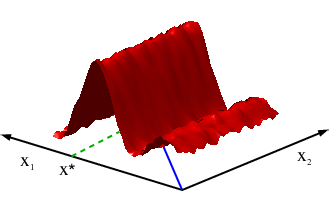
\includegraphics[width=0.5\textwidth]{images/highdim_images/Random embeddings in a nutshell1.png}
    \end{figure}
    \end{column}
\end{columns}
    \pause
    \begin{columns}[T]
    \begin{column}{0.45\linewidth}
    \vspace{-1em}
    \item Subspace $x_1=x_2$ is guaranteed to include the optimum.
        \end{column}
        \begin{column}{0.5\linewidth}
    \begin{figure}
    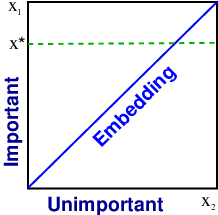
\includegraphics[width=0.5\textwidth]{images/highdim_images/Random embeddings in a nutshell2.png}
    \end{figure}
    \end{column}
\end{columns}
    \pause
\begin{columns}
\begin{column}{0.45\linewidth}
    \vspace{-8em}
    \item Idea applies to any $d$-dimensional linear subspace
    \item Let's us scale to arbitrary $D$ (e.g., $D=1$ billion)
\end{column}
\begin{column}{0.5\linewidth}

\end{column}
\end{columns}
\end{itemize}


\end{frame}

%----------------------------------------------------------------------
\begin{frame}[c]{Random Embedding Bayesian Optimization (REMBO)}
\begin{columns}[T]
\begin{column}{0.5\textwidth}
\begin{itemize}
    \item Generate a random matrix $A \in \realnum^{D \times d}$
    \item Choose a bounded region set $\boobsspace\subset\realnum^d$
    \item Use BO to optimize $g(\conf)=\cost(\pmb{Ay})$ instead of high dimensional $\cost(\conf)$
\end{itemize}
\end{column}
\begin{column}{0.5\textwidth}
\begin{figure}
    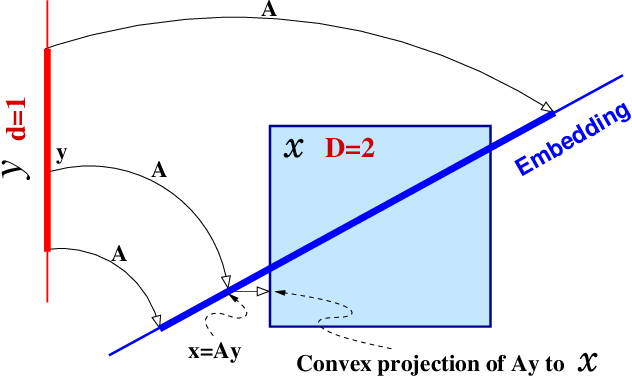
\includegraphics[width=0.8\textwidth]{images/highdim_images/Embedding.png}
\end{figure}
\end{column}

\end{columns} 
\end{frame}

%----------------------------------------------------------------------

%----------------------------------------------------------------------
\begin{frame}[c]{REMBO- Pseudocode}


\begin{algorithm}[H]
    %\DontPrintSemicolon
    \LinesNumbered
    \SetAlgoLined
    \setcounter{AlgoLine}{0}
    
    \textcolor{blue}{Generate a random matrix $\pmb{A} \in \realnum^{D\times d}$}\\
    \textcolor{blue}{Choose the bounded region set $\boobsspace\subset\realnum^d$}\\
    Initialize $\dataset_{0}$ as $\emptyset$.\\
    \For{$t=1,2,...$}{
        Find \textcolor{blue}{$\bonextobs \in \realnum^{d}$} by optimizing the acquisition function $\acq$:
        \textcolor{blue}{$\bonextobs=\argmax_{\pmb{y}\in\boobsspace} \acq(\pmb{y}|\dataset_{t})$}.
        Augment the data $\dataset_{t+1}=\dataset_{t} \cup \{(\textcolor{blue}{\pmb{y}_{t+1},f(\pmb{A}\pmb{y}_{t+1}))}\}$.\\
        Update the kernel hyper-parameters.
        }
    
    \caption{REMBO: Bayesian Optimization with Random Embedding. Blue text denotes parts that are changed compared to standard Bayesian Optimization.}
\end{algorithm}
\end{frame}
%----------------------------------------------------------------------
\begin{frame}{Random Embedding Bayesian Optimization-Summary}
\begin{columns}[T] % align columns
\begin{column}{.48\textwidth}


    \begin{block}{Advantages}
    \begin{itemize}
    	\item Exploits low effective dimensionality 
    	\item Allows scaling to very high dimensions
    	\item Applies to both continuous and categorical variables
    	\item Trivial modification of BO algorithm
    	\item Coordinate independent (invariant under rotations)
    \end{itemize}
    \end{block}
\pause
\end{column}%

\hfill%

\begin{column}{.48\textwidth}

    \begin{block}{Disadvantages}
    \begin{itemize}
    	\item Sensitive to the definition of the bounded low dimensional constrained space $\boobsspace$
    	\item Assumes truly unimportant dimensions
    	%Limits a high dimensional function in a low dimensional embedding
    	%\item Sensitive to the effective dimension
    \end{itemize}
\end{block}

\end{column}
\end{columns}   
\end{frame}

%----------------------------------------------------------------------
%\subsection{High dimensional BO via additive models}
\begin{frame}{High Dimensional Bayesian Optimisation and Bandits via Additive Models}
\vspace{2em}
\begin{itemize}
    \item Recall:

    \begin{itemize}
        \item Standard GPs do not tend to fit well in high dimensions
        \item Maximizing the acquisition function is also computationally challenging
        \pause
    \end{itemize}
\medskip
    \item Idea:
    \begin{itemize}
        \item Assume additive structure of the objective function
        \begin{equation*}
            f(\conf)=f^{(1)}(\conf^{(1)})+f^{(2)}(\conf^{(2)})+...+f^{(M)}(\conf^{(M)})
        \end{equation*}
        \item Use an alternative acquisition function which applies to an additive kernel
    \end{itemize}
\end{itemize}

\end{frame}

%----------------------------------------------------------------------
\begin{frame}{Additive GP Models in a nutshell}
        \begin{equation*}
            f(\conf)=f^{(1)}(\conf^{(1)})+f^{(2)}(\conf^{(2)})+...+f^{(M)}(\conf^{(M)})
        \end{equation*}
\begin{itemize}
\begin{columns}[T]
\begin{column}{0.45\linewidth}

\hspace{2em}
    \item Key assumption: $f$ decomposes into lower-dimensional additive components $\conf^{(j)} \in \pcs^{(j)}, j \in \{1,..,M\}$
    \item The decompositions are disjoint $\conf^{(i)} \cap \conf^{(j)} = \varnothing$
    \pause
    \item Each decomposition $f^{(j)}(\conf^{(j)})$ is modelled by an individual GP
    \pause
    \end{column}
    \begin{column}{0.45\linewidth}
        \begin{figure}
    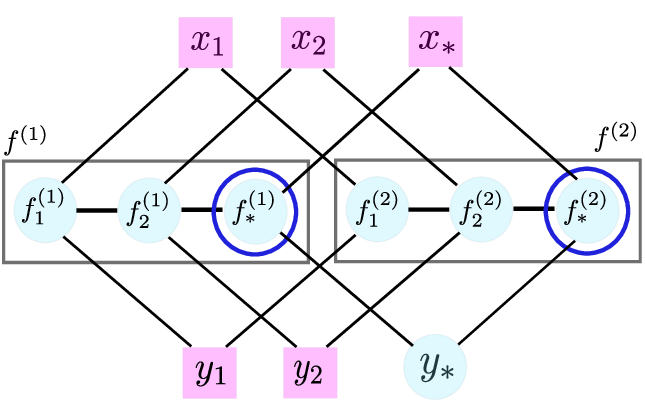
\includegraphics[width=0.7\textwidth]{images/highdim_images/additive-models.png}
    \caption{Decomposition in two additive components (M=2)}
    \end{figure}
    \end{column}
\end{columns}
\end{itemize}
\end{frame}
%----------------------------------------------------------------------
\begin{frame}{Additive GP-UCB}
\begin{itemize}

    \item Idea: Represent acquisition function as sum of functions on decompositions:
    \begin{equation*}
        \acq_{t}(\conf) = \sum_{j}\acq_{t}^{(j)}(\conf^{(j)})
    \end{equation*}
\pause
\medskip    
    \item $\acq_{t}$ is maximized by maximizing each $\acq_{t}^{(j)}$ separately:
    \begin{equation*}
        \hat{\varphi}_{t}^{(j)}(\conf^{(j)}) = \mean_{t-1}^{(j)}(\conf^{(j)}) + \beta_{t}^{1/2}\stddev_{t-1}^{(j)}(\conf^{(j)})
    \end{equation*}
\end{itemize}
\end{frame}


%----------------------------------------------------------------------

\begin{frame}{Additive GP-UCB- Pseudocode}
\begin{algorithm}[H]
    %\DontPrintSemicolon
    \LinesNumbered
    \SetAlgoLined
    \setcounter{AlgoLine}{0}
    \SetKwInOut{Input}{Input}
    
    %\Input{Kernels $\kernel^{(1)},...,\kernel^{(M)}$, Decomposition $(\pcs^{(j)})_{j=1}^{M}$}\\
    \Input{ Kernels $\kernel^{(1)},...,\kernel^{(M)}$, Decomposition $(\pcs^{(j)})_{j=1}^{M}$
    $\dataset_{0}\leftarrow\varnothing$}
    \For{$j=1,...,M$, $(\mean_0^{(j)},\kernel_0^{(j)})\leftarrow(0,\kernel^{(j)})$.}{
        \For{$j=1,...,M$,}{
            $\confI{t}_{(j)}\leftarrow\argmax_{z\in\pcs^{(j)}}\mean_{t-1}^{(j)}(z) +\sqrt{\beta_{t}}\stddev_{t-1}^{(j)}(z)$;\
            
            $\confI{t}\leftarrow\bigcup_{j=1}^{M} \confI{t}_{(j)}$;\
            
            $\boobs\leftarrow$ Query $\cost$ at $\confI{t}$;\
            
            $\dataset_{t}=\dataset_{t-1}\cup\{(\confI{t},\boobs)\}$;\
            
            Perform Bayesian Optimization posterior updates conditioned on $\dataset_{t}$ to obtain $\mean_{t}^{(j)},\stddev_{t}^{(j)}$ for $j=1,...,M$;\
        }
    }
    \caption{Add-GP-UCB}
\end{algorithm}
\end{frame}


%----------------------------------------------------------------------
\begin{frame}{High dimensional BO via additive models-Summary}
\begin{columns}[T] % align columns
\begin{column}{.48\textwidth}


    \begin{block}{Advantages}
    \begin{itemize}
    	\item Exploits low effective dimensionality
    	\item Scales GP-UCB to high dimensional parameter spaces
    	\item Regret is linearly dependent on the dimension D when $\cost$ is additive
    	\item Add-GP-UCB applies to an additive kernel
    \end{itemize}
    \end{block}
\pause
\end{column}%

\hfill%

\begin{column}{.48\textwidth}

    \begin{block}{Disadvantages}
    \begin{itemize}
    	\item Relies on structural assumptions about the objective function
    	\item Restricted to an axis aligned representation
    	\item Sensitive on the number of additive components
    \end{itemize}
\end{block}

\end{column}
\end{columns}   
\end{frame}

%---------------------------------------------------------------------
%\subsection{Random Forests}
\begin{frame}{Random Forests}
%\note{We're not 100\% sure whether SMAC should be in the methods for high-dimensional problems?}
BO with random forests as surrogates has been shown to perform well in high dimensions:
\begin{itemize}
    \item Can handle complex parameter spaces:
    \begin{itemize}
        \item High dimensionality (low effective dimensionality)
        \item Mixed continuous/discrete parameters
        \item Conditional parameters
    \end{itemize}
\pause
\smallskip
    \item Can handle non-standard noise
    \begin{itemize}
        \item Non-Gaussian noise
        \item Heteroscedastic noise
    \end{itemize}
\pause
\smallskip
    \item Effective model for off-the-shelf Bayesian optimization
    \begin{itemize}
        \item Robustness of the model
        \item Model overhead
    \end{itemize}
\pause
\smallskip
    \item SMAC is a Bayesian optimization tool that uses random forests as a surrogate model
\end{itemize}
\end{frame}


%----------------------------------------------------------------------


